\subsection{Qualità di processo - Analisi dei requisiti}

\vspace{0.3cm}

\subsubsection{M18PROS - Percentuale di requisiti obbligatori soddisfatti}

\vspace{0.3cm}

\begin{figure}[H]
    \centering
    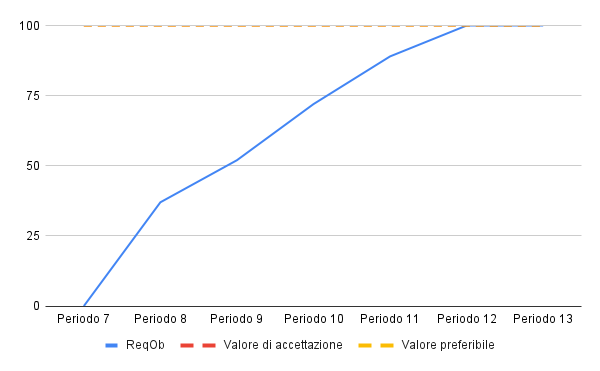
\includegraphics[width=0.9\textwidth]{../Images/PianoDiQualifica/PROS.png}
    \caption{Proiezione della copertura dei requisiti obbligatori soddisfatti nei vari periodi di progetto.}
    \label{fig:10}
\end{figure}

\vspace{0.2cm}

\textbf{PB}: La rappresentazione grafica evidenzia l’adempimento completo, pari al 100\%, dei requisiti obbligatori nel periodo più recente. L’attuazione di tali requisiti ha avuto inizio nel periodo immediatamente successivo alla fase di progettazione del sistema, poiché era imprescindibile disporre di una comprensione accurata dell’architettura da implementare.

\subsubsection{M19PRDS - Percentuale di requisiti desiderabili soddisfatti}

\vspace{0.3cm}

\begin{figure}[H]
    \centering
    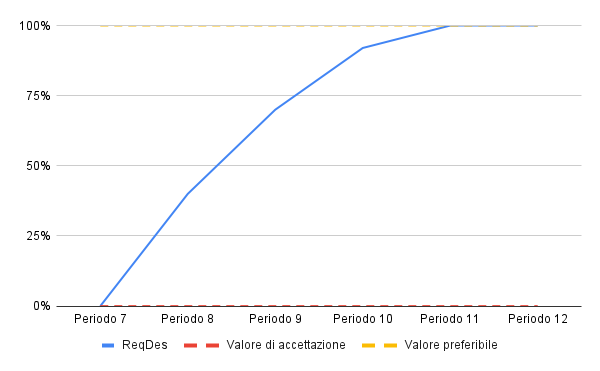
\includegraphics[width=0.9\textwidth]{../Images/PianoDiQualifica/PRDS.png}
    \caption{Proiezione della copertura dei requisiti desiderabili soddisfatti nei vari periodi di progetto.}
    \label{fig:11}
\end{figure}

\vspace{0.2cm}

\textbf{PB}: La rappresentazione grafica evidenzia anche in questo caso, l'adempimento completo, pari al 100\%, dei requisiti desiderabili nel periodo più recente. La soddisfazione di tali requisiti è stata possibile grazie alla loro implementazione in un momento successivo rispetto ai requisiti obbligatori e all’incoraggiamento alla realizzazione da parte della proponente, in quanto considerata una funzionalità ritenuta utile per l’utente finale.

\subsubsection{M20PRPS - Percentuale di requisiti opzionali soddisfatti}

\vspace{0.3cm}
\begin{figure}[H]
    \centering
    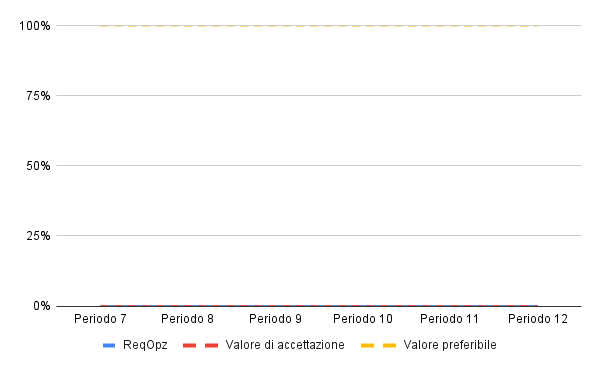
\includegraphics[width=0.9\textwidth]{../Images/PianoDiQualifica/PRPS.png}
    \caption{Proiezione della copertura dei requisiti desiderabili soddisfatti nei vari periodi di progetto.}
    \label{fig:12}
\end{figure}

\vspace{0.2cm}

\textbf{PB}: La rappresentazione grafica evidenzia, con dispiacere, l’insoddisfazione complessiva dei requisiti opzionali. L’omissione nell’implementazione di tali requisiti è attribuibile alla priorità conferita ai requisiti obbligatori e desiderabili, che hanno necessitato di un impegno considerevole. È fondamentale enfatizzare che l’omissione nell’implementazione di tali requisiti è stata concordata con la proponente.